\def\QRCODE{TB_image_TUT.IMG.segmentation_region_growing_matlabqrcode.png}
\def\QRPAGE{http://www.iptutorials.science/tree/master/TB_image/TUT.IMG.segmentation_region_growing/matlab}
\mcorrectionsection{Matlab correction}

The tricky part of this code is that, for convenience, some Java code is used inside matlab. This can be really useful when using particular structures and objects like lists, queues, etc.

\begin{matlab}
% needs an image I, gray level
% double is needed to perform comparison
I = double(imread('cameraman.tif'));
[Sx, Sy] = size(I);
imshow(I,[]);

% seed
[x, y]=ginput(1);
seed = round([y;x]); % beware of inversion of coordinates

I(seed(1), seed(2))

% create the queue structure by a Java object
queue = java.util.LinkedList;

% Visited matrix : result of segmentation
% this matrix will contain 1 if in the region, 
%                         -1 if visited but not in the region, 
%                          0 if not visited.
visited = zeros(size(I));
\end{matlab}

The next code is used to compute the visited matrix and display it.
\begin{matlab}
% Start of algorithm ----------------------
queue.add(seed); 
visited(seed(1), seed(2)) = 1;

tic
while ~queue.isEmpty()
   p = queue.remove();
   
   % look at the pixel in a 8-neighborhood
   r = p(1); % row
   c = p(2); % col
   for i=max(1,r-1):min(Sx,r+1)
       for j=max(1,c-1):min(Sy,c+1)
           if (visited(i,j)==0) % not visited yet
               if (predicate(I, [i j], seed, visited)) 
						% condition is fulfilled
                    visited(i, j) = 1;
                    queue.add([i;j]); % add to visiting queue
               else
                   visited(i, j) = -1;
               end
           end
       end
   end
end
toc
% end of the algorithm: 
% the visited matrix contains the segmentation result

figure(); imshow(visited==1,[]);
\end{matlab}

%\FloatBarrier

Notice that values $-1$ of the \minline{visited} matrix avoid testing multiple times the same pixel. In the predicate function, the \minline{visited} matrix is used in case of adapting the predicate to the current region. In the next case, the candidate pixel's graylevel is compared to the mean gray value of the region. The results are illustrated Fig.\ref{fig:regiongrowing:matlab:cameraman}.

\begin{matlab}
function r = predicate2(I, p, seed, visited)
% threshold parameter
t = 10;

m = mean(I(visited==1));
if abs(I(p(1), p(2)) - m) <= t
    r = true;
else
    r = false;
end
\end{matlab}


Another predicate function would be:
\begin{matlab}
function r = predicate3(I, p, seed, visited)
% threshold parameter
t = 10;

m = mean(I(visited==1));
sigma = std(I(visited==1));
if abs(I(p(1), p(2)) - m) <= t * (1-sigma/m)
    r = true;
else
    r = false;
end
\end{matlab}

\begin{figure}[htbp]
\centering
\subfloat[Original image.]{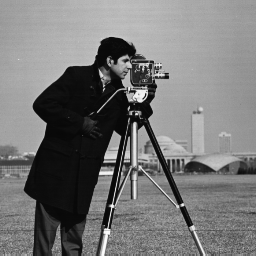
\includegraphics[width=.45\linewidth]{cameraman.png}}\hfill
\subfloat[First predicate function.]{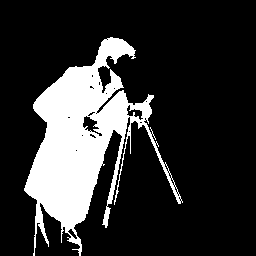
\includegraphics[width=.45\linewidth]{predicate_seg.png}}

\subfloat[Second predicate function.]{
\includegraphics[width=.45\linewidth]{predicate2_seg.png}}\hfill
\subfloat[Third predicate function.]{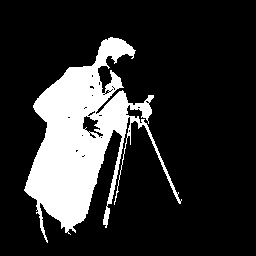
\includegraphics[width=.45\linewidth]{predicate3_seg.png}}
 
\caption{The segmentation result highly depend on the order used to populate the queue, on the predicate function and on the seed pixel. The seed pixel is chosen somewhere in the coat of the cameraman.}
\label{fig:regiongrowing:matlab:cameraman}
\end{figure}
